\chapter{Sediment transport}
\label{chap:Transporte-Sedimentos}
    The sediment transport is the movement of solid particles, carried by a fluid over a distance, flowing in the same direction. The transport is a combination of action of gravity on the system and the fluid forces, mainly the fluid drag force. A vast number of phenomena are related to the fluid transport, such as in industrial processes (when transporting ores through a pipeline), or the transformation of landscapes (in the formation or disappearance of dunes) \cite{Granular_Media_Between_Fluid_and_Solid}. The different fluids acts differently, resulting in phenomena like: pluvial erosion, river erosion and silting, all caused by water; and phenomena caused by wind, like dunes and desertification. 

    The types of transport can be classified as shown in Figure \ref{fig:transport_mode}, in which sediments are removed from one location and deposited into another, in different temporal and spatial scales. A formation can appear on the scale of minutes from a few centimetres high on the bottoms of rivers and oceans, to geological formations thousands of years old and hundreds of kilometres long.

\begin{figure}[H]
    \centering
    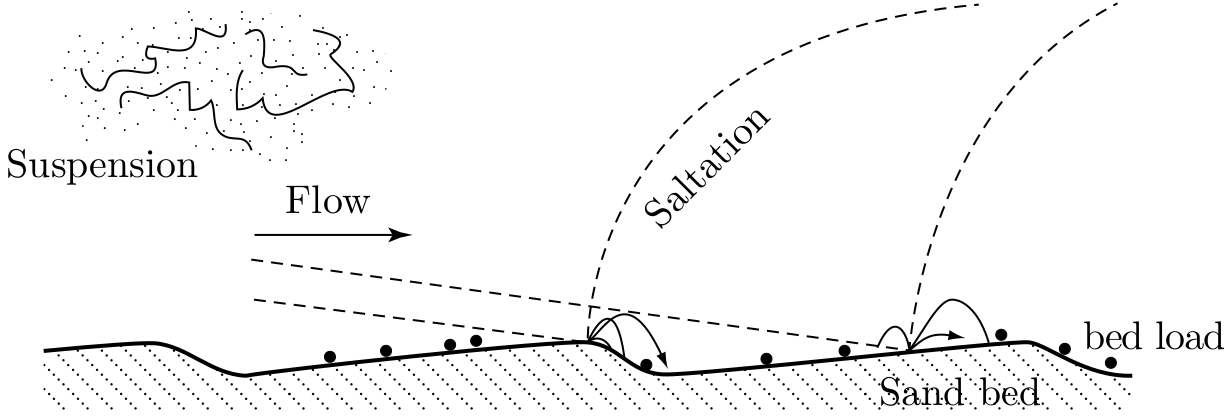
\includegraphics[width = 0.75 \textwidth]{04-figuras/TransportModes.png}
    \caption[Transport modes.]{Schematic diagram of different transport modes. Figure taken from \cite{Granular_Media_Between_Fluid_and_Solid}.}
    \label{fig:transport_mode}
\end{figure}

    Solid materials can be transported by the following modes: bedload, which is the transport of material rolling over a thin layer of the granular base and occurs when the gravitational force is the most prevalent force in the system \cite{Bedforms_in_a_turbulent_stream}. Bedload can occur on the bottom of streams and lakes and on the surface of a land. Saltation is the transport mode of materials that collides with the granular base in jumps, occurring when gravitational and drag forces are the most relevant in the system, and can be seen in rivers and in wind erosive processes. Finally suspension is the transport mode of materials in which the drag forces caused by turbulent fluctuations become the order of magnitude of the grain weight and dominate the dynamics of the system \cite{FVSCS}. Suspension may be observed in sandstorms or when sweeping house dust. 

    Single-phase models are not able to reproduce the physics involved in this problem. Models of granular materials without the presence of fluid do not exhibit the properties of transport modes such as bedload, saltation and suspension. Likewise, fluid models without sediments are not able to describe the deposition, erosion or even saturation properties. Therefore, it is necessary that the model has the two phases described, sediment and fluid. 

    Two intrinsic properties of drag are the saturation length scale $L_\textrm{sat}$ and the saturation time scale $T_\textrm{sat}$. The saturation length scale quantifies the characteristic distance for the grains to have the maximum density transported by the fluid $q_\textrm{sat}$. The saturation time scale, on the other hand, indicates the characteristic time for the transported material density to decay when the fluid velocity decreases sharply, or for the transported material density to increase when the fluid velocity increases sharply \cite{Granular_Media_Between_Fluid_and_Solid}. The main transport governing equation is the Transport Equation, which relates the quantities:
\begin{equation}
    T_\textrm{sat} \frac{\partial q}{\partial t} + L_\textrm{sat} \frac{\partial q}{\partial x} = q_\textrm{sat} - q,
    \label{equ:transporte}
\end{equation}
where $T_{sat}$ is the saturation time that flux takes to adjust, $L_{sat}$ is the saturation length that flux takes to adjust, $q_{sat}$ is the saturated flux, $q$ is the flux, $t$ is the time and $x$ is the direction of the flux.

    Aiming at a model capable of reproducing such characteristics, the use of DEM combined with the use of FDM simulate the behavior of grains and fluid, interacting with different approaches to continuous fluid and discrete to granular material. 

    To describe the interactive behavior between fluid and granular material, we will use computer simulations based on the work of Dr. Philippe Claudin \cite{Numerical_simulation_of_turbulent_sediment_transport, Sand_ripples_and_dunes, Direct_numerical_simulations_of_aeolian_sand_ripples}. By imposing the initial conditions of the fluid, the time needed for the new regime to reach stationary conditions is measured. The number of grains flowing through the system, in the steady state, provides the saturated volumetric flow $q_\textrm{sat}$, which serves as a parameter for comparing and measuring the saturation time and the saturation length. The process is repeated for each input parameter, thus quantifying the different transitions between modes of transport.

\begin{figure}[H]
    \centering
    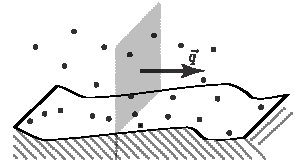
\includegraphics[width=0.65\textwidth]{04-figuras/flux_density.pdf}
    \caption[Transport volumetric flux.]{A schematic of the volumetric flux $q$. Figure taken from \cite{Granular_Media_Between_Fluid_and_Solid}.}
    \label{fig:flux_density}
\end{figure}

    The saturated flux $q_\textrm{sat}$ is the main quantity we analyze the sediment transport. It measures the volume of the particles crossing a vertical surface of unit transverse size per unit time. The definition is as it follows:
\begin{equation}
    q_\textrm{sat} = \frac{1}{A \phi_b} \frac{\pi}{6}d^3 \sum_p u^p,
    \label{equ:qsat}
\end{equation}
where $A$ is the surface area that particles cross, $\phi_b$ is the packing fraction of the base, $d$ is the average grain diameter and $u^p$ is the grain velocity.

    Other two quantities related to the saturated flux is the number of of transported grains per unit area $n$ and the mean grain horizontal velocity $u_p$:
\begin{equation}
    n = \frac{\left(\sum_p u_p\right)^2}{A\sum_p {u_p}^2}
    \label{equ:n}
\end{equation}
\begin{equation}
    \bar{u}_p = \sum_p \frac{\sum_p {u_p}^2}{\sum_p {u_p}}
    \label{equ:up}
\end{equation}
and the relation between $q_\textrm{sat}$, $n$ and $\bar{u}_p$ is:
\begin{equation}
    q_\textrm{sat} = \frac{1}{\phi_b} \frac{\pi}{6} d^3 n \bar{u}_p.
\end{equation}

\section{Threshold}
    To describe the bedload transportation threshold, we are going to write the momentum equations in steady state ($\sum F = 0$) and find the values where they get balanced, for the maximum velocity of the fluid lays the grains in rest. So, the forces that will hold grains statically until moving are given by:
\begin{equation}
    m\frac{\partial u_p}{\partial t} = F_{Drag} + F_{Friction},
\end{equation}
where the acceleration of the particle is $m\frac{\partial u_p}{\partial t} = 0$, due to the steady state regime, $F_{Drag}$ is the drag force, $F_{Friction}$ is the friction force.

\begin{equation}
    F_{Drag} = 3\pi \rho_f \nu d\left(u_f-u_p\right),
\end{equation}
is the drag force onto grains, where $\rho_f$ is the density of the fluid, $\nu$ is the viscosity of the fluid, $d$ is the diameter of the grain, $u_f$ is the fluid velocity and $u_p$ is the grains velocity.

\begin{equation}
    F_{Friction} = -\mu_s F_{Gravity},
\end{equation}
is the friction force, and is dependent of the gravity, where $\mu_s$ is the static friction coefficient, related to the Coulomb friction.

\begin{equation}
    F_{Gravity} = \frac{\pi}{6}d^3\left(\rho_p-\rho_f\right)g,
\end{equation}
is the gravity force onto the grains, where $\rho_p$ is the grains density and $g$ is the gravitational acceleration.

    And since we know that the fluid shear stress is given by:
\begin{equation}
    \tau_f = \rho_f \nu \frac{\partial u_f}{\partial z},
\end{equation}
where $\tau_f$ is the fluid shear stress, these equations combined and considering the fact that only the upper half of the particle feels drag force\footnote{As the upper layer of grains are in rest, the fluid flows more in this upper layer of grains, and almost vanish below it.}, we have:
\begin{equation}
    u_f = \frac{\tau_f}{\rho_f\nu}\frac{d}{2}.
\end{equation}
while $u_p = 0$.

    Using the Shields number (Equation \ref{equ:Shields}) and manipulating previous equations, when applied drag force is equals to friction force, we can find the threshold by:
\begin{equation}
    \Theta_t = \frac{2}{9}\mu_s,
\end{equation}
the $\Theta_t$ is the threshold that grains flow. Below this threshold grains do not move, while above it grains flows with the fluid.

\section{Contribution of moving grains}
    To introduce the contribution of the moving grains, we are still going to use most of the previous calculation. Still, particles have reached steady state, so $m\frac{\partial u_p}{\partial t} = 0$ is still valid. Considering that grains are moving, we have the balance force:
\begin{equation}
    0 = F_{Drag} + F_{Friction} + F_{Grains},
\end{equation}
now $F_{Grains}$ is the force due to the moving grains, where it is:
\begin{equation}
    F_{Grains} = \frac{\rho_p d^3 u_p \tau_p d^2}{d^2/\nu},
\end{equation}
where $\rho_p d^3 u_p$ is the momentum carried by moving grains, $\tau_p$ is the grains shear stress and $d^2/\nu$ is the characteristic time to this viscous contact dynamics.

    Looking to the limit just after the threshold, one can get a discontinuity on the grains velocity, and we expect for this behaviour an abrupt change on the friction coefficient, once we change from static regime to moving regime. Then we rewrite equations to include this term:
\begin{equation}
    \frac{3}{2}\pi\rho_f\nu d u_p = \frac{3}{2}\pi\rho_f\nu d u_f - \mu_d \frac{\pi}{6}d^3 \left(\rho_p-\rho_f\right)g,
\end{equation}
where $\mu_d$ is the new friction coefficient. Then, rewriting $u_p = v_0$ just in the limit after the threshold, we have:
\begin{equation}
    v_0 = \frac{2}{9}\left(\mu_s-\mu_d\right)v_b,
\end{equation}
where $v_b = \sqrt{\left(\frac{\rho_p}{\rho_f}-1\right)gd}$ is the normalised velocity by the grains parameters.

    Now, the grains shear stress is:
\begin{equation}
    \tau_p \propto n,
\end{equation}
where $n$ is the number of moving grains by the cross section parallel to the fluid flow divided by the area of this cross section. From previous analysis, we quantify $n$, $\overline{u}_p$ and $q$ as following:
\begin{subequations}
    \begin{empheq}{align}
        n = a_n \left( \Theta - \Theta_t \right) \frac{1}{d^2},\\
        \overline{u}_p = \mathcal{G} \, \frac{\Theta - \Theta_t + u_0}{1 - a_u \left( \Theta - \Theta_t \right)} \, u_b,\\
        q_\textrm{sat} = \frac{1}{\phi_b} \frac{\pi}{6} d^3 n \overline{u}_p,
    \end{empheq}
    \label{equ:flux_steadystate_model}
\end{subequations}
where $n$ is the number of transported grains per unit area, $a_n$ is the adjusted parameter to the data present in Figure \ref{fig:TM_profiles}(d), $\Theta$ is the Shields number, $\Theta_t$ is the threshold where transportation happens, $d$ is the average grain diameter, $\overline{u}^p$ is the mean grain horizontal velocity, $\mathcal{G}$ is the Galileo number, $u_0$ is the adjusted velocity to the data present in Figure \ref{fig:TM_profiles}(d), $a_u$ is the adjusted parameter to the data present in Figure \ref{fig:TM_profiles}(d), $u_b = \sqrt{\mathcal{D}_{R}gd}$ is the normalized velocity by the grains parameters, $q$ is the the volume of the particles (at the bed density) crossing a vertical surface of unit transverse size per unit time.
